\section{Introduction}
\label{sec:introduction}

Computer vision and natural language processing models have become increasingly powerful through the use of large-scale training data. Recent models such as CLIP~\cite{Radford2021LearningTV}, DALL-E~\cite{Ramesh2021ZeroShotTG}, GPT-3~\cite{Brown2020LanguageMA}, and Flamingo~\cite{flamingo} use massive amounts of task agnostic data to pre-train large neural architectures that perform remarkably well at downstream tasks, including in zero and few-shot settings. In comparison, the Embodied AI (\eai) research community predominantly trains agents in simulators with far fewer scenes~\cite{Ramakrishnan2021HabitatMatterport3D,kolve2017ai2,Deitke2020RoboTHORAO}. Due to the complexity of tasks and the need for long planning horizons, the best performing \eai models continue to overfit on the limited training scenes and thus generalize poorly to unseen environments.


In recent years, \eai simulators have become increasingly more powerful with support for physics, manipulators, object states, deformable objects, fluids, and real-sim counterparts \cite{kolve2017ai2,savva2019habitat,Shen2020iGibsonAS,Gan2020ThreeDWorldAP,xiang2020sapien}, but scaling them up to tens of thousands of scenes has remained challenging. Existing \eai  environments are either designed manually \cite{kolve2017ai2,Gan2020ThreeDWorldAP} or obtained via 3D scans of real structures \cite{savva2019habitat,Ramakrishnan2021HabitatMatterport3D}. The former approach requires 3D artists to spend a significant amount of time designing 3D assets, arranging them in sensible configurations within large spaces, and carefully configuring the right textures and lighting in these environments. The latter involves moving specialized cameras through many real-world environments and then stitching the resulting images together to form 3D reconstructions of the scenes. These approaches are not scalable, and expanding existing scene repositories multiple orders of magnitude is not practical.

We present \env, a framework built off of AI2-THOR~\cite{kolve2017ai2}, to procedurally generate fully-interactive, physics-enabled environments for \eai research. Given a room specification (e.g., a house with 3 bedrooms, 3 baths, and 1 kitchen), \env can produce a large and diverse set of floorplans that meet these requirements (Fig.~\ref{fig:examples}). A large asset library of 108 object types and 1633 fully interactable instances is used to automatically populate each floorplan, ensuring that object placements are physically plausible, natural, and realistic. One can also vary the intensity and color of lighting elements (both artificial lighting and simulated skyboxes) in each scene, to simulate variations in indoor lighting and the time of the day. Assets (such as furniture and fruit) and larger structures such as walls and doors can be assigned a variety of colors and textures, sampled from sets of plausible colors and materials for each asset category. Together, the diversity of layouts, assets, placements, and lighting leads to an arbitrarily large set of environments -- allowing \env to scale orders of magnitude beyond the number of scenes currently supported by present-day simulators. In addition, \env supports dynamic material randomizations, whereby colors and materials of individual assets can be randomized each time an environment is loaded into memory for training. Importantly, in contrast to environments produced using 3D scans, scenes produced by \env contain objects that both support a variety of different object states (\eg open, closed, broken, \etc) and are fully interactive so that they can be physically manipulated by agents with robotic arms. We also present \elienv, a 3D artist-designed set of 10 high quality fully interactable houses, meant to be used as a test-only environment for research within household environments. In contrast to AI2-iTHOR (single rooms) and RoboTHOR (lesser visual diversity) environments, \elienv contains larger, diverse, and realistic houses.
% supporting a variety of object states and agents with arms that can navigate around and manipulate objects.


\begin{figure}[tp]
    \centering
    \vspace{-0.35in}
    \makebox[\textwidth][c]{
        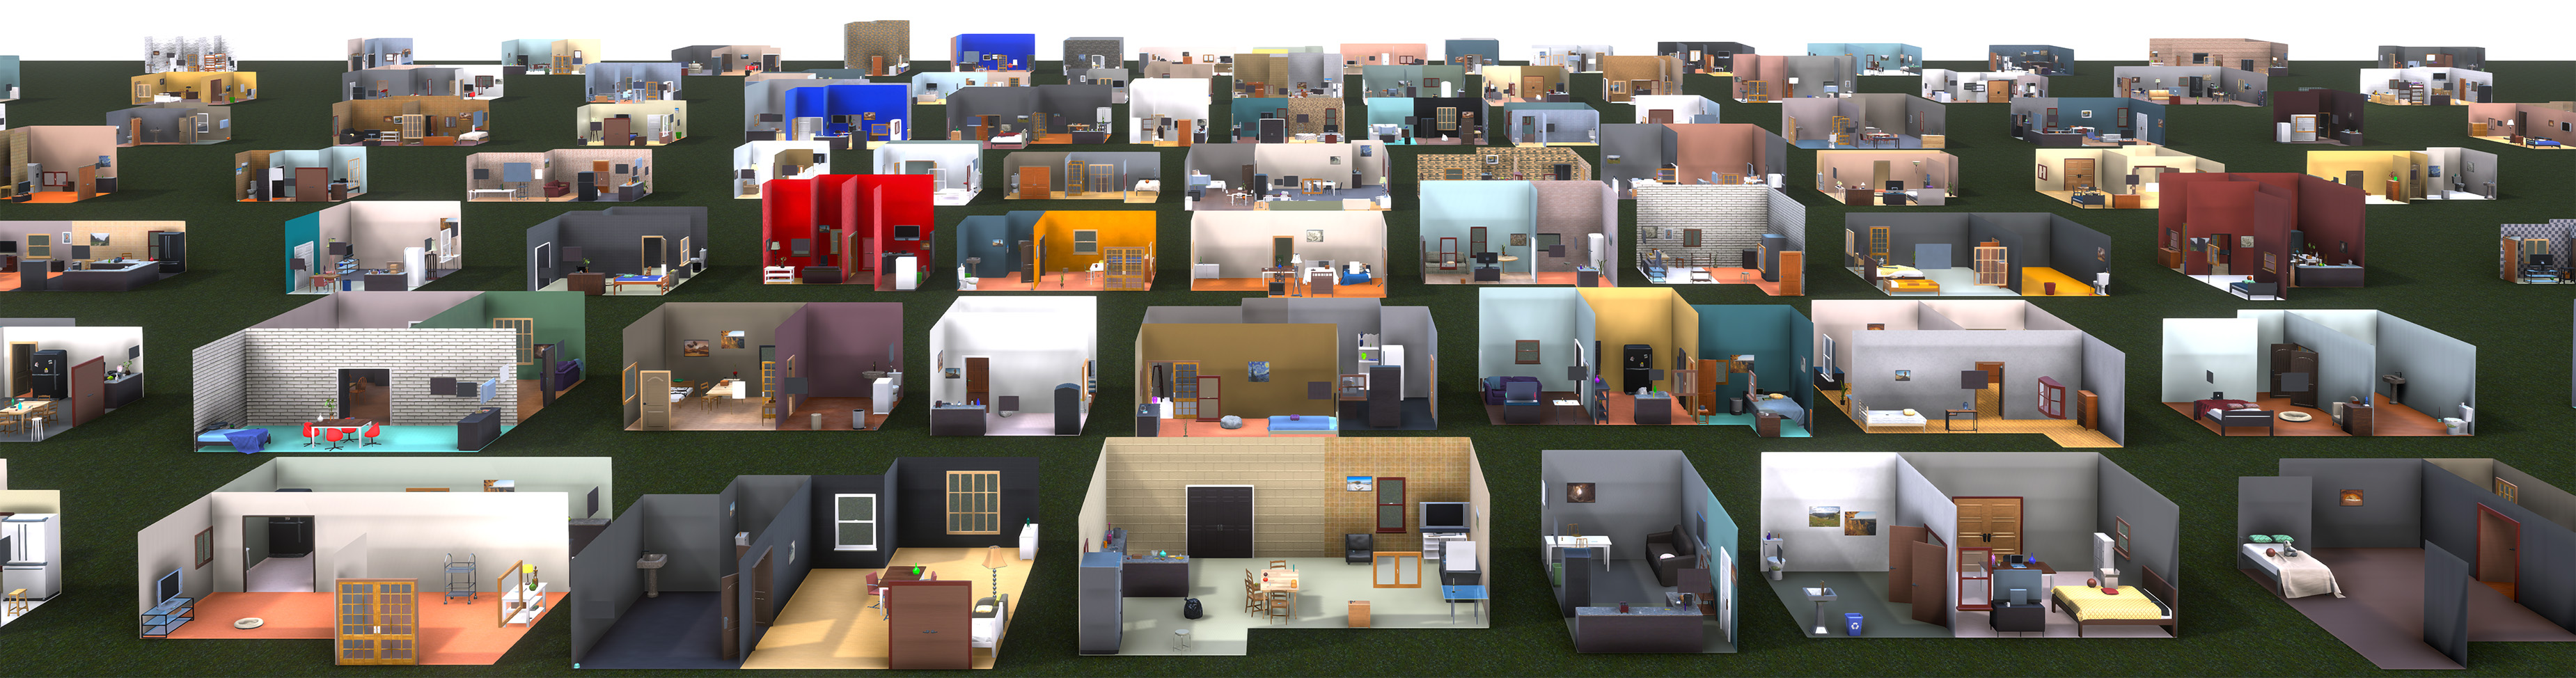
\includegraphics[width=1\textwidth]{figures/procthor-cover.jpg}
    }
    \caption{We propose \env{}, a framework to procedurally generate a large variety of diverse, interactable, and customizable houses.}
    \vspace{-0.2in}
    \label{fig:examples}
\end{figure}

We demonstrate the ease and effectiveness of \env by sampling an environment of 10,000 houses (named \tenk), composed of diverse layouts ranging from small 1-room houses to larger 10-room houses. We train agents with very simple neural architectures (CNN+RNN) -- \emph{without} a depth sensor, and instead only employing RGB channels, with no explicit mapping and no human task supervision -- on \tenk and produce state-of-the-art (SoTA) models on several navigation and interaction benchmarks. As of 10am PT on June 14th, 2022 we obtain (1) \textbf{RoboTHOR ObjectNav Challenge}~\cite{robothor-challenge} --  0-shot performance superior to the previous SoTA which uses RoboTHOR training scenes -- with fine-tuning we obtain an 8.8 point improvement in SPL over the previous SoTA; (2) \textbf{Habitat ObjectNav Challenge 2022}~\cite{habitat-challenge} -- top of the leaderboard results with a ${>}3$ point gain in SPL over the next best submission; (3) \textbf{1-phase Rearrangement Challenge 2022}~\cite{roomr-challenge} -- top of the leaderboard results with Prop Fixed Strict improving from 0.19 to 0.245; (4) \textbf{AI2-iTHOR ObjectNav} -- 0-shot numbers which already outperform a previous model that trains on AI2-iTHOR, with fine-tuning we achieve a success rate of 77.5\%; (5) \textbf{ArmPointNav}~\cite{manipulathor} -- 0-shot number that beats previous SoTA results when using RGB; and (6) \textbf{ArchitecTHOR ObjectNav} -- a large success rate improvement from 18.5\% to 31.4\%. Finally, an ablation analysis clearly shows the advantages of scaling up from 10 to 100 to 1K and finally to 10K scenes and indicates that further improvements can be obtained by invoking \env to produce even larger environments.

In summary, our contributions are (1) \env, a framework that allows for the performant procedural generation of an unbounded number of diverse, fully-interactive, simulated environments, (2) \elienv, a new, 3D artist-designed set of houses for \eai evaluation, and (3) SoTA results across six \eai benchmarks covering manipulation and navigation tasks, including strong 0-shot results.
\env will be open-sourced and the code used in this work will be released.  

